---
layout: post
title:  "Accuracy of diagonal mouse paths"
categories: assignment
background: '/img/posts/accuracyMouse/banner.jpg'
date:   2021-05-18 8:00:00 +0200
published: true
---
\documentclass{article}
\usepackage{graphicx}
\usepackage{amsmath}
\usepackage{caption}
\usepackage{subcaption}
During our day-to-day life we constantly use computers. Programs should be ergonomically optimized to increase speed, and therefore efficiency, when using the program. This can be done by improving the accuracy of the user when using the program. One meassurement of accuracy is the width of the user's mouse path when using the program. During this research the focus was specifically put on laptop users, as this is where improvements to accuracy can easily be made. The main point of research was if laptop users are just as accurate in diagonal mouse paths as in straight mouse paths. So in the case of designing programs for laptop users, should certain mouse path angles  be preferred or avoided? So; Do laptop users on average have the same accuracy with a diagonal mouse path compared to a straight mouse path? 

\section*{Methods}
The dataset used for this experiment was a mouse test done by students at the Eindhoven University of Technology. Outliers of the dataset were removed, by only keeping the 99th percentile of the data, whilst keeping maximum data. Further cleaning of the data, and checking for equal distrubution, was not neccesary as the size of the dataset is large enough (>13000). For this experiment, only trackpad users were selected as this is the group where the highest gain in efficiency can be achieved. All paths were either grouped into a ‘Diagonal’ or ‘Straight’ angle types. As the mouse experiment only had 8 directions, 4 straight and 4 diagonal with equal chances, the data was equally distrubuted. To compare the means of these groups, a one-sided less t-test was used.  

\begin{figure}
    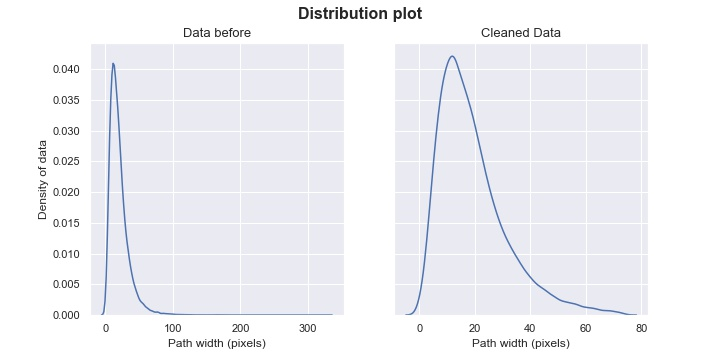
\includegraphics[width=\textwidth]{/img/posts/accuracyMouse/Distribution.jpeg}
    \caption{Distrubution of the data before and after taking the 99th percentile}
\end{figure}

\section*{Hypothesis}
For the hypothesis the null hypothesis is taken to be that the average width of the paths straight and diagonal are the same. For the null hypothesis to be rejected, the alternative hypothesis should apply that the average width of diagonal paths is significantly higher than the average of the straight paths. For it to be significantly higher the p-value of the t-test should be lower than 0.05.

  $$H_0: \mu_{width straight} = \mu_{width diagonal}$$
  $$H_a: \mu_{width straight} < \mu_{width diagonal}$$

\begin{figure}
	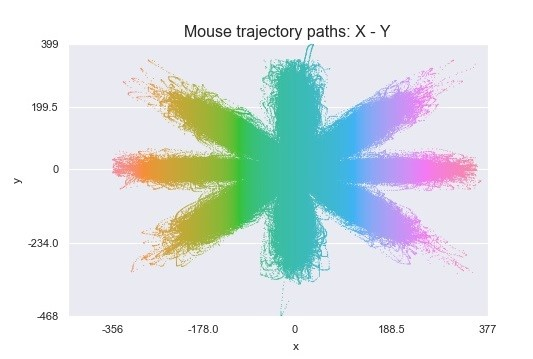
\includegraphics{/img/posts/accuracyMouse/pathsEdited.jpeg}
	\caption{Mouse trajectory paths - all trials}
\end{figure}

% \begin{figure}
% 	\centering
%     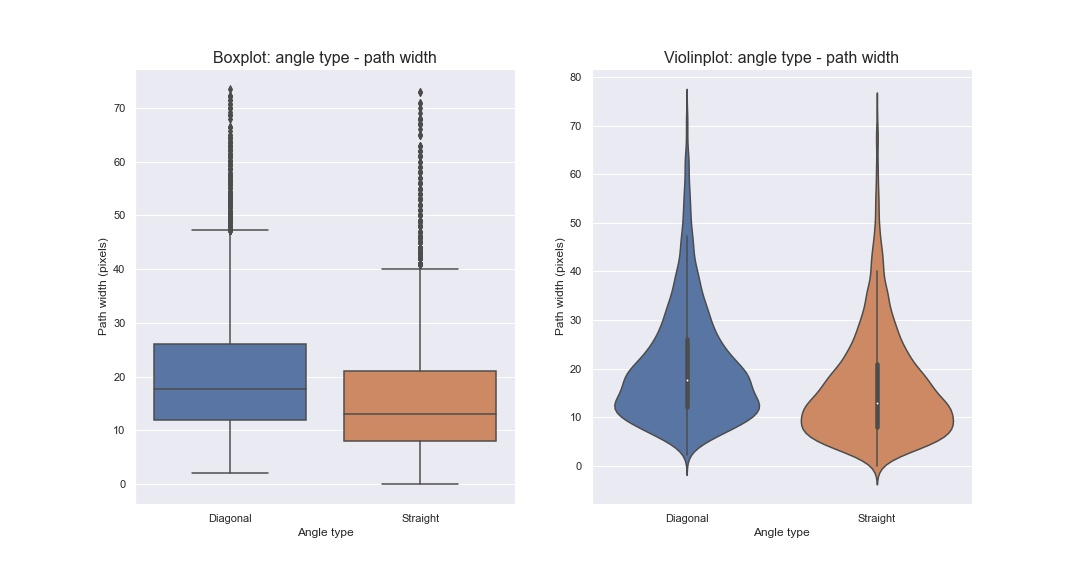
\includegraphics{/img/posts/accuracyMouse/plotAngle.jpeg}
%     \label{fig:angle}
% \end{figure}



\section*{Discussion}
The mouse trajectory paths shows trajectories in all directions, so there are no direction assumptions. The dataset has a length of more than thirteen thousand and is large enough. Even still the length of the dataset is large, the cleaned also follows a distribution curve. For all these reasons, the one-sided two-sample t-test for a lesser mean is valid and applied. 
\begin{equation*}
  p_{value} = 5.193 * 10^{-97}
\end{equation*}

The p-value is (a lot) smaller than an alpha of 0.05, for a 95\% confidence interval. The null hypothesis ($𝐻_0$) is rejected, and the alternative hypothesis ($H_a$) is accepted.

\section*{Conclusion}
The null hypothesis ($𝐻_0$) is rejected based on that the p-value is much smaller than an alpha of 0.05, and the alternative hypothesis ($𝐻_𝑎$) is accepted. Meaning, the mean width of trajectories that are straight is lower, and the mean of diagonal trajectories are larger. Trackpad users are less accurate for diagonal trajectories. For using a program, this means that diagonal trajectories should be avoided to aid in maximising accuracy and therefor efficiency.

An example of such a program which is ergonomically optimized is Photoshop by Adobe. When using Photoshop the user often has to switch tools by selecting a different one with the cursor in on of the toolbars. These toolbars are situated at straight angles from the working are, highlighted in red in the figure below. By using straight angles in such a work optimized program as Photoshop, the efficiency and accuracy of the user is increased.

\begin{figure}
    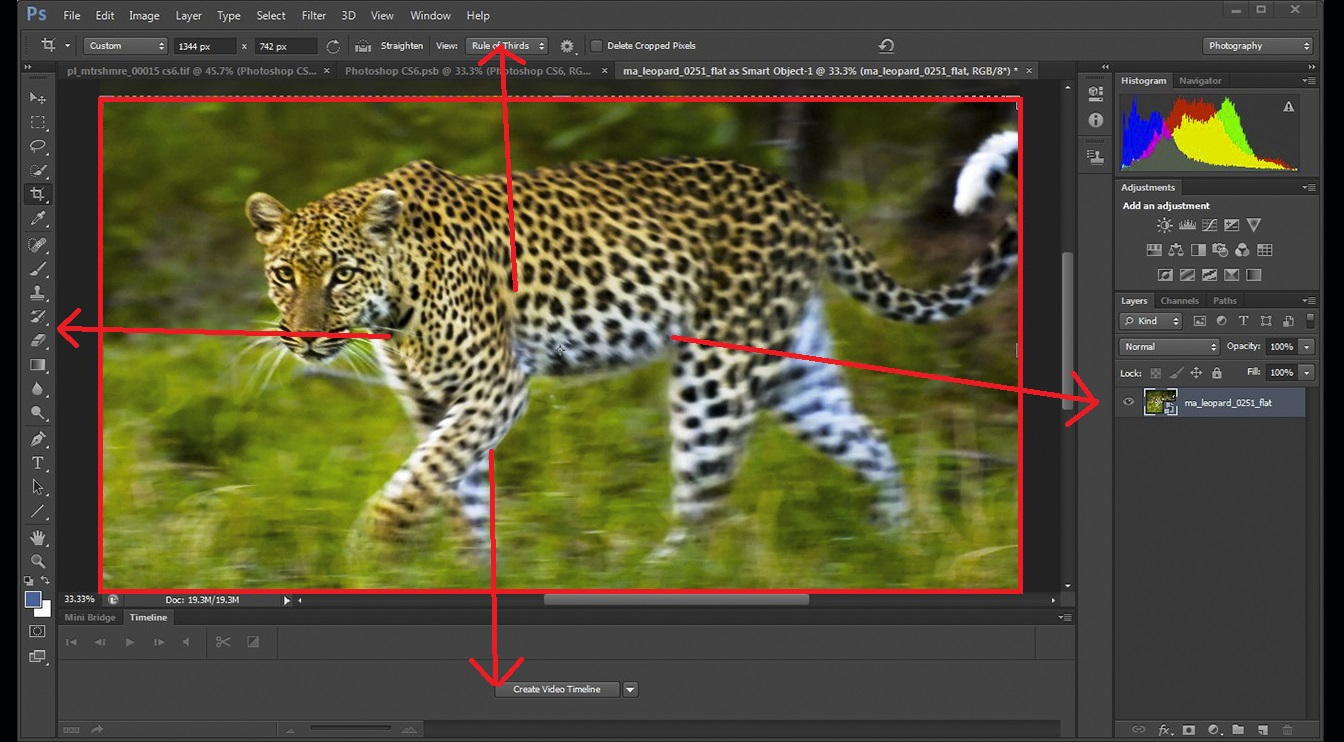
\includegraphics[width=\textwidth]{/img/posts/accuracyMouse/Photoshop-CS6.jpg}
    \caption{Photoshop - \href{https://www.extremetech.com/extreme/123179-photoshop-cs6-plenty-of-goodies-for-everyone}{Extremetech}}
\end{figure}